\subsection{Background}
The most popular type of wearable in 2019 is the smartwatch \cite{best_watches}. 
Smartwatches are devices worn on one's wrist, equipped with sensors, and in some 
cases wireless communication capability for syncing data to a smartphone. They have
rich operating systems (OS), on-board processors and memory, and come in a wide range
of varieties from basic to high-end, with different specialized models in between \cite{smartwatch_arch_rit}.

% ======= TYPICAL SMARTWATCH SPECIFICATIONS =============
\subsection{Typical Specifications}
Modern smartwatches typically have similar components to computers, albeit at a much smaller scale.
They have an OS, which is most cases is proprietary to the manufacturer (i.e. watchOS for Apple);
a single- or dual-core processor ranging from 80MHz to over 1.2GHz depending on the type of watch;
up to a gigabyte of memory; battery life ranging between 18 hours to over a week; and depending on 
the watch - sensors to measure heart rate, fitness statistics, 
and atmospheric pressure \cite{smartwatch_arch_rit}.

It is simple to build a system that can accommodate all the required features of a smartwatch
using normal computing components, however the challenge with a smartwatch is weight, size, and power
consumption, as it needs to fit comfortably on the wrist, and be able to record data for at least
an entire day on a single charge. This means all components must be lightweight, and energy efficient.
According to ARM, the most necessary optimizations are using small data memories, using slower clock
speeds, and choosing a silicon process technology that will offer the lowest possible power consumption,
meaning the biggest design trade-off when designing smartwatches is between performance and 
power consumption \cite{arm_wearable}. To examine these trade-offs, two popular smartwatches will be
analyzed for the architecture decisions that went into their design and manufacturing.

% ANALYZING APPLE AND GARMIN
\subsection{Analysis of Examples}
Two popular examples of smartwatches are the Apple Watch Series 5,
and the Garmin Forerunner 235, both shown below in Figure \ref{watches:pictures}.
These devices are priced quite differently, carry different levels of functionality, and are
therefore targeted towards different market segments. Shown below in Table \ref{watch:price} are 
prices for the watches listed above \cite{apple_price} \cite{garmin_price}.

% Figure of watches
\begin{figure}[h]
    \centering
    \begin{subfigure}{.5\textwidth}
      \centering
      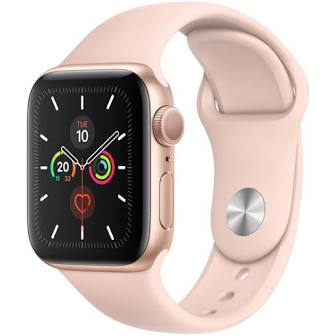
\includegraphics[width=.4\linewidth]{media/apple_pic.jpeg}
      \caption{Apple Watch Series 5 \cite{apple_price}}
      \label{fig:sub1}
    \end{subfigure}%
    \begin{subfigure}{.5\textwidth}
        \centering
        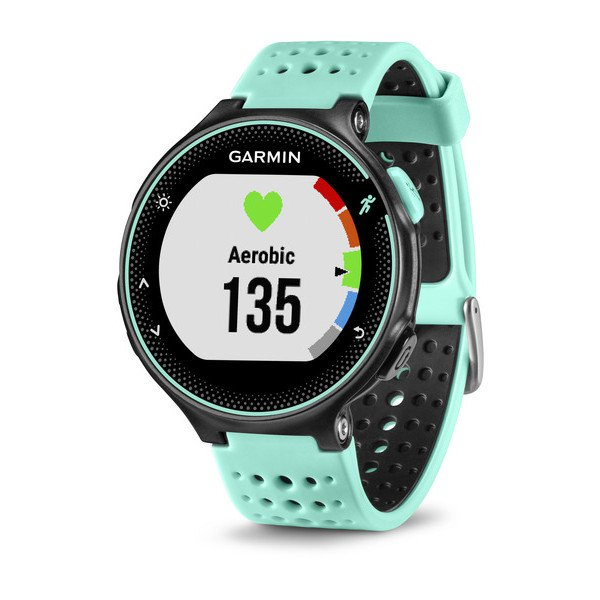
\includegraphics[width=.4\linewidth]{media/garmin_pic.jpeg}
        \caption{Garmin Forerunner 235 \cite{garmin_price}}
        \label{fig:sub3}
      \end{subfigure}
    \caption{Smartwatches discussed in this report.}
    \label{watches:pictures}
\end{figure}

% Watch prices table
\begin{table}[h]
    \centering
    \caption{Smartwatch Prices}
    \csvautotabular{data/prices.csv} 
    \label{watch:price} 
\end{table}

Clearly, these watches come at different price points, target different segments of the market, and
of course come with different architectures for accommodating the necessary features in each model. This
section will cover each of the watches shown above in greater detail.

% ========= APPLE WATCH ===============
\subsubsection{Apple Watch Series 5}
% APPLE WATCH BACKGROUND
\paragraph{Background}
The Apple Watch Series 5 is the newest iteration of smartwatch from Apple Inc., released in September
2019. Priced at \$529, clearly this is considered a higher-end smartwatch, fitting in with Apple's
other product lines (iPhone, iPad, and Mac). This watch weighs between 30-40g depending the case, it
has all-day battery life, a touch screen (324x394), voice call, GPS, compass, and music streaming capabilities,
as well as the ability to run thousands of apps from the Apple App Store made specifically 
for the Apple Watch \cite{apple_specs}. This device is made for Apple users, as it requires 
an iPhone to make use of all its features. Its operating system is the Apple-designed watchOS.

Much of what makes the Apple Watch quite appealing is the variety of sensor technology that can track
much of your health and fitness data. This sensor technology will be discussed, along with other
computer architecture components in this section.

\paragraph{Hardware and Functionality}
An innovation brought on by the Series 5 is the always-on display, a first for Apple Watch.
An always-on display is not ideal for a device wanting low-power consumption, especially a high-resolution
screen with a high refresh rate like the one on the Apple Watch. However, this new model incorporates
a low temperature poly-silicon and oxide (LTPO) display which reduces the refresh rate of the watch's
screen from 60Hz to 1Hz, the minimum frequency for the always-on display to accurately 
display the time \cite{apple_specs}. This is a clever way to reduce power consumption by reducing frame
rate when the watch is not being used interactively. 

The processor and System in Package (SiP) at the core of the Apple Watch Series 5 is Apple's S5 chip,
shown below in Figure \ref{fig:s5chip}. This is the fifth iteration of their custom-designed 
smartwatch chip where the entire system is fabricated into a single component with a footprint
of about 40mm. This SiP includes 32GB of storage, the memory, as well some the sensors that come with the 
Series 5, including its GPS component and magnetometer (compass) \cite{apple_specs}.

% APPLE S5 CHIP FIGURE
\begin{figure}[h]
    \centering
    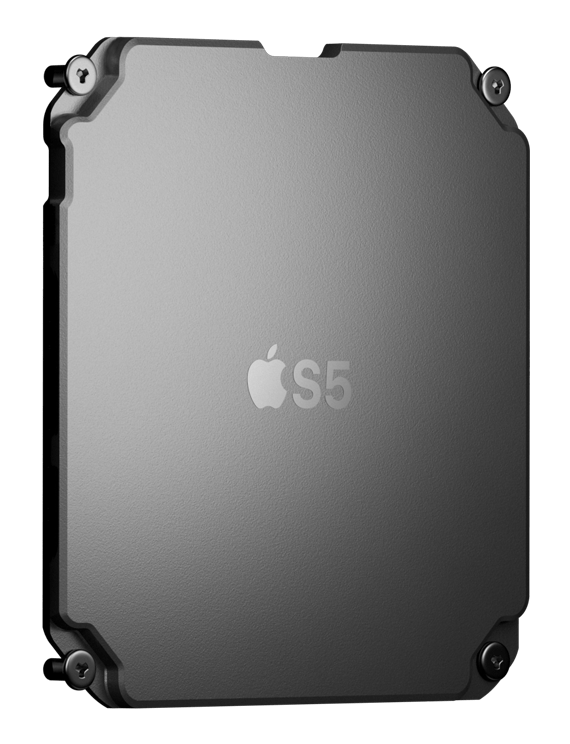
\includegraphics[width=.15\linewidth]{media/apple_s5_chip.png}
    \caption{Apple S5 Processor \cite{apple_s5_pic}}
    \label{fig:s5chip}
\end{figure}
% END APPLE S5 CHIP FIGURE

The Series 5 incorporates other sensors whose data is processed. These sensors are an electric
heart rate sensor, which constantly monitors heart rate, and can perform an electrocardiogram 
(ECG/EKG) almost as accurate as a single-lead EKG \cite{apple_health}. Data from this sensor can
be monitored and programmed to alert the wearer if there is any abnormal heart activity. The watch
also uses its microphone to monitor noise levels, and alerts the user when current noise exposure could
pose a risk for long-term hearing damage. 

Arguably the most important sensors on a smartwatch with fitness tracking capabilities are the accelerometer,
which actually tracks the motion patterns of the watch itself based on acceleration forces \cite{accel_expl},
and the gyroscope. Data from GPS, accelerometer, gyroscope, heart rate monitor, and your own personal 
health data (height, weight, age) are
used together to give you valuable insights into your workouts. The Series 5 comes with pre-programmed
sports like cycling, running, swimming, and yoga, amongst others. In running activities, the watch
tracks and can display your calories burnt, your pace, your heart rate, your distance, cadence, and
elapsed time \cite{apple_fitness}. Having this data displayed in real time on your wrist, and available for analysis after the
run is something that makes this device so valuable, as it helps people stay motivated and quantitatively
monitor their improvements.

\paragraph{Apple Watch Summary}
After analyzing the price-point, features, and specifications of the Apple Watch Series 5, it is clear
this is a high-end wearable device that values performance highly for a wearable device. It has a battery
that needs to be recharged each night, and while it carries valuable stats for many different workouts,
this app is targeted at individuals who want to exercise to remain healthy, and not so much professional
athletes or athletes who need high-performance functionality for hours at a time (ultra-marathoners and
Iron-man Triathletes), as the battery would exhaust itself before the workout finishes, as using all sensors
(especially GPS) for extended periods depletes battery life rapidly \cite{apple_battery}. Therefore, this
wearable device's main purpose is to allow for smartphone-like functionality on your wrist.

% =========== GARMIN =================
\subsubsection{Garmin Forerunner 235}
\paragraph{Background}
If its name wasn't obvious enough, the Garmin Forerunner 235 is first and foremost a runner's
watch. It weighs 42g, and has a slightly larger footprint than the Apple Watch, fitting in a 45mm square.
It costs \$319.99, which is significantly less expensive than the Apple Watch Series 5. Battery life using
it without GPS functionality is 9 days, whereas one charge gives 11 hours of GPS usage. The display (215x180)
is not touch screen, navigation is done with buttons on the side. It can connect and 
sync data to a smartphone, but it can also be used independent of any other device. The sensors 
in this device include GPS, heart rate monitor, and an accelerometer \cite{garmin_price}. 
It run's Garmin's own proprietary smartwatch OS \cite{garmin_specs}.

What makes the Forerunner appealing is the trade-offs it makes in comparison with the Apple Watch
for specializing the device to be a pure running wearable. These specializations and optimizations will
be discussed in this section.

\paragraph{Hardware and Functionality}
Please note due to the lack of resources about the Forerunner 235's internal hardware,
the information provided here is for the Forerunner 230, which is the same as the 235
but with the absence of a heart rate monitor \cite{forerunner230235}.

According to Rich Nass' teardown of the Garmin Forerunner 230, the core microprocessor
is the Atmel Smart SAMG53 (ATSAMG53), as shown below in Figure \ref{fig:garmTear} \cite{forerunner_teardown}.

\begin{figure}[h]
    \centering
    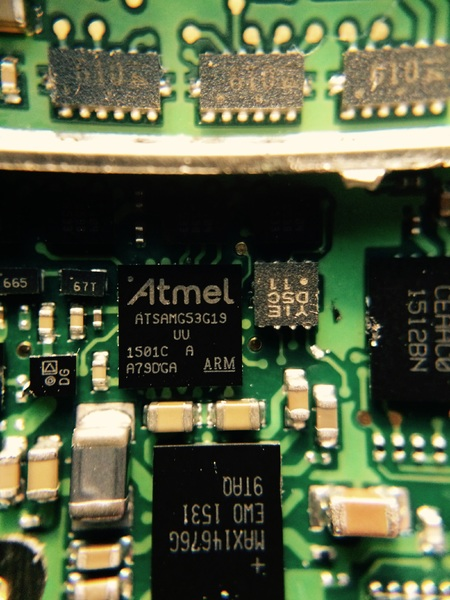
\includegraphics[scale=0.6]{media/garmin_teardown.jpg}
    \caption{The Atmel microprocessor at the core of the Forerunner \cite{forerunner_teardown}.}
    \label{fig:garmTear}
\end{figure}

The ATSAMG53 chip is built with the ARM Cortex-M4 core with a three-stage pipeline,
with 96kB of SRAM on the instruction/data (I/D) bus (for I/D cache), 
up to 512kB of embedded Flash memory, includes a floating point unit 
(FPU), and a maximum CPU speed of 48 MHz \cite{atmel_specs}.

Like the Apple Watch, the Forerunner comes pre-loaded with activities, but is primarily focused on
running and cycling \cite{garmin_price}. It takes many of the same running metrics as the Apple Watch,
like cadence, pace, heart rate, and distance, as shown in Figure \ref{fig:garm_disp}. 
However, the Forerunner can do so for longer periods due to a lower power consumption.
An interesting feature built into the Forerunner is the ability to load "courses" onto the watch and have
the GPS guide you through turn-by-turn \cite{garmin_course}. The Apple Watch does not offer this without downloading a third-party
application, which likely uses more power than built-in functionality.

\begin{figure}[h]
    \centering
    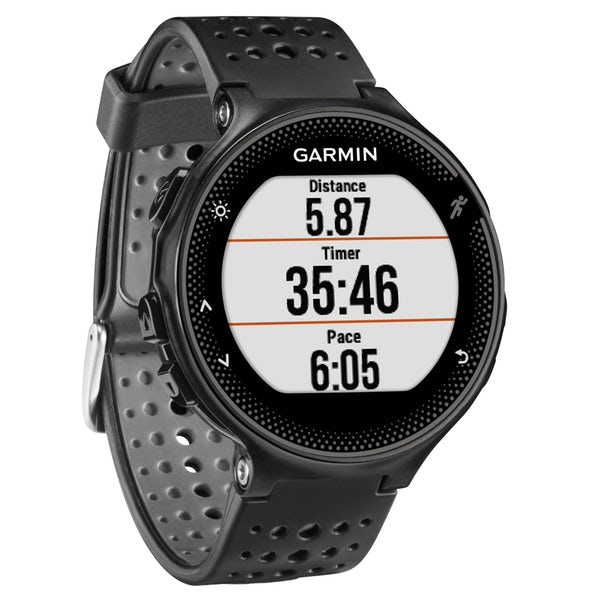
\includegraphics[scale=0.25]{media/garmin_running.jpg}
    \caption{Mid-run display on Forerunner displaying distance, time, and current pace.}
    \label{fig:garm_disp}
\end{figure}

\paragraph{Garmin Forerunner 235 Summary}
It is clear that the Garmin Forerunner does not attempt to be the "smartphone on your wrist" that the Apple
Watch offers. The Forerunner is an energy efficient wearable that is specialized for tracking running
activities. It is not meant for people who wants lots of functionality in their smartwatch, but for people
looking for a reliable, efficient watch they can use for their fitness tracking and not have to charge every
single day. Therefore, the Garmin Forerunner 235 is an example of how power consumption is prioritized over
performance in the power-performance trade-off of wearables, as functionality is optimized to only have the
necessities.

\subsection{Smartwatch Summary}
Comparing as contrasting the Apple Watch Series 5 and Garmin Forerunner 235 is an insightful case study
for different varieties of smartwatches. It illustrates different trade-offs between performance and
power consumption, and shows how regardless of the type of wearable, the footprint of the hardware, and
power consumption are the two most important design criteria and constraints.